\section{Task 3 - Just an ordinary box}

\begin{frame}{Task 3 - Just an ordinary box}
    \begin{itemize}
        \item Create a stateless widget called Box. It should:
        \begin{itemize}
            \item have a width and a height of 200dp (default unit).
            \item have a boolean (bool) property "active"
            \item if active, it should be green and have a text saying "Active"
            \item if inactive, it should be gray and a Text saying "Inactive"
        \end{itemize}
        \item Place a box on the second screen.
        \item Make it so that when you click on the box, it changes from active to inactive (remember GestureDetector?)
        \item It should be inactive by default
    \end{itemize}
\end{frame}


\begin{frame}{Task 3 - Just an ordinary box}
    \begin{columns}
        \begin{column}{0.5\textwidth}
            \begin{figure}[h]
                {
                    \setlength{\fboxsep}{0pt}%
                    \setlength{\fboxrule}{0.5pt}%
                    \fbox{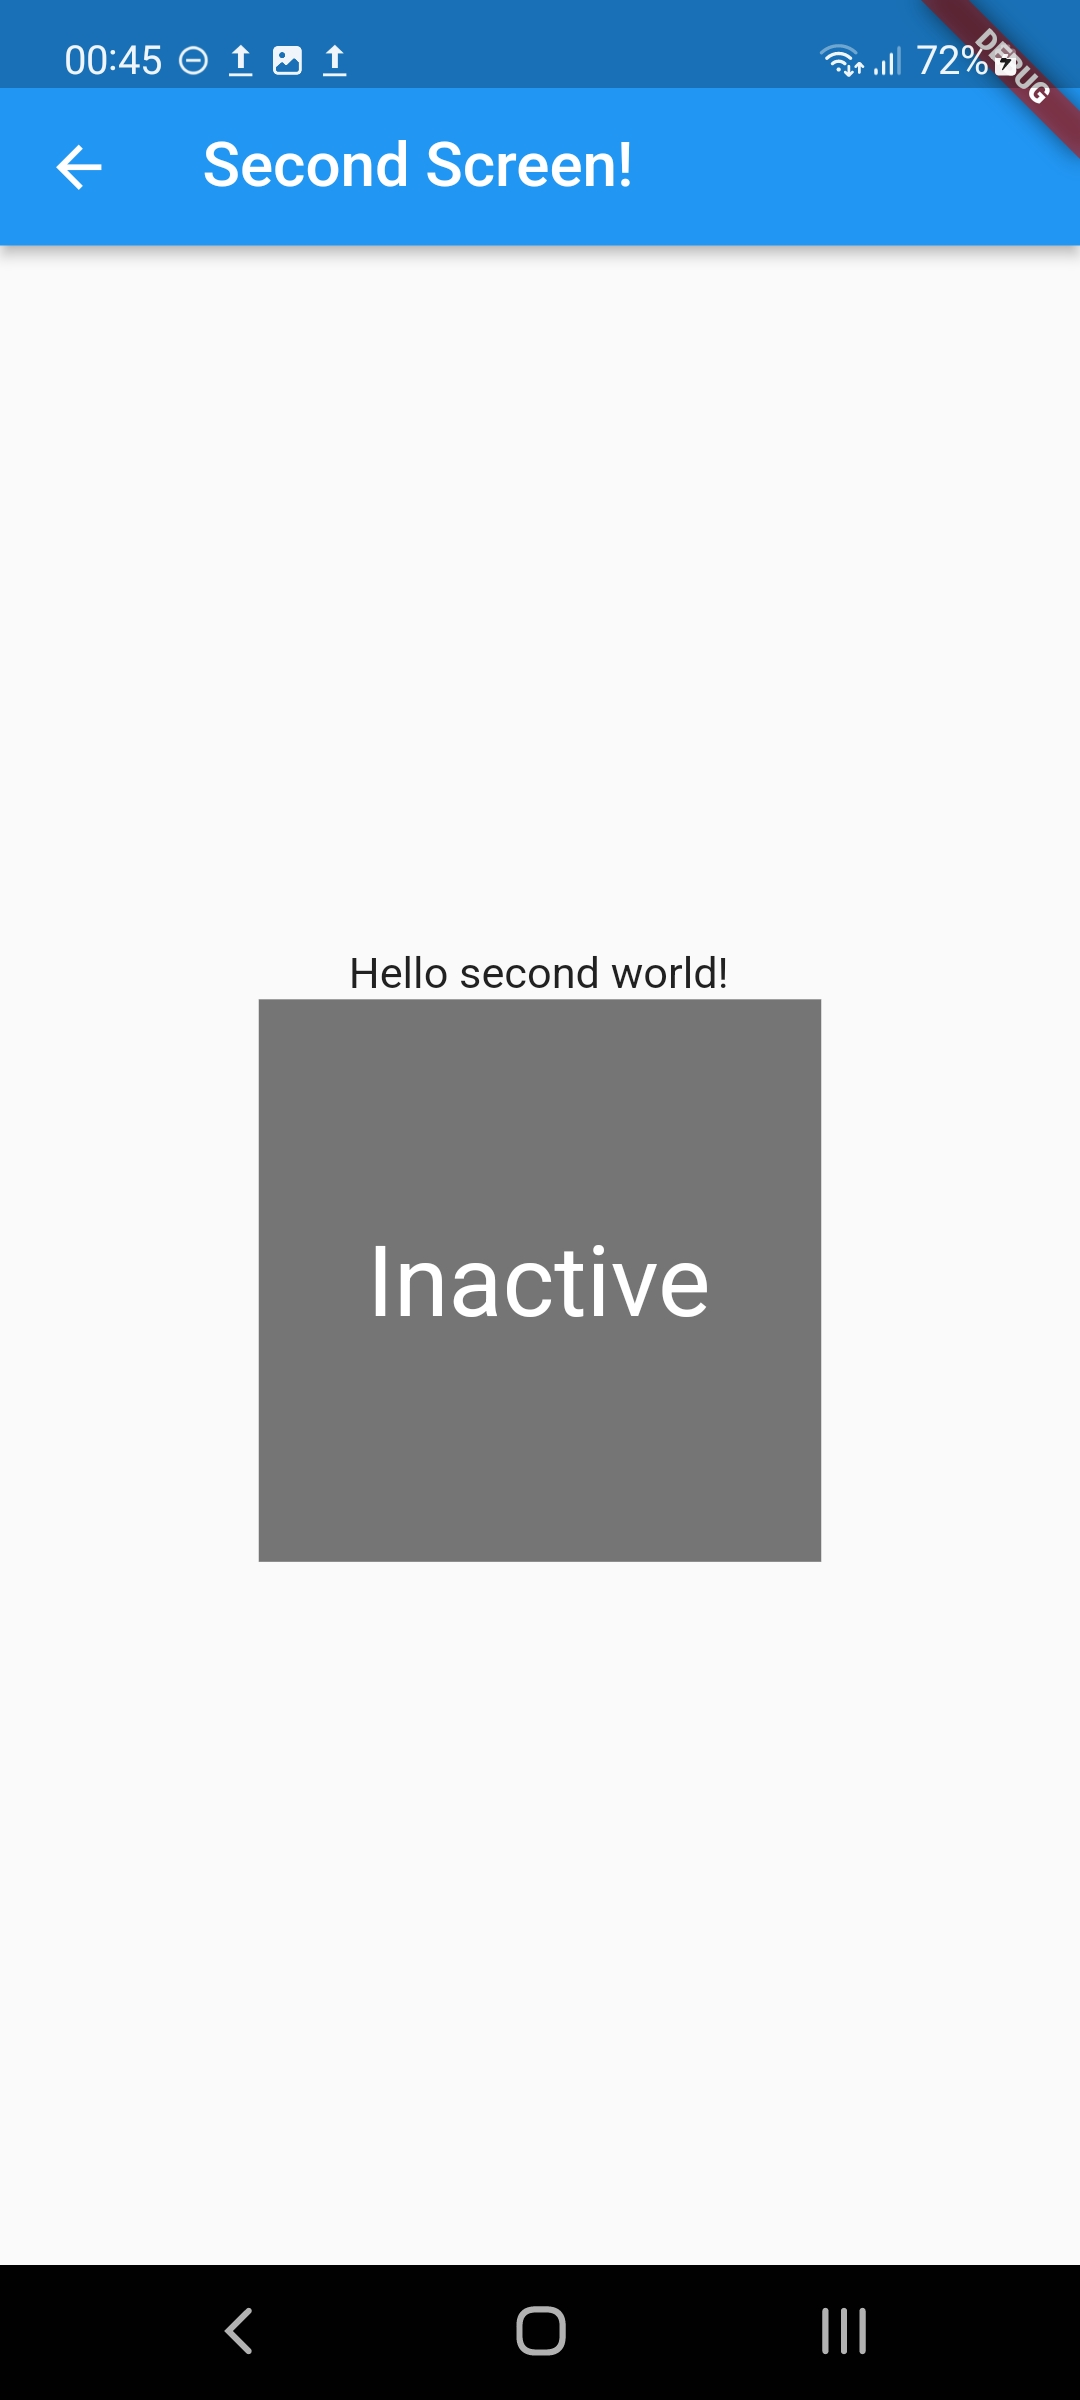
\includegraphics[width=0.5\textwidth]{images/task3-1.jpg}}
                }
            \end{figure}
        \end{column}
        \begin{column}{0.5\textwidth}
            \begin{figure}[h]
                {
                    \setlength{\fboxsep}{0pt}%
                    \setlength{\fboxrule}{0.5pt}%
                    \fbox{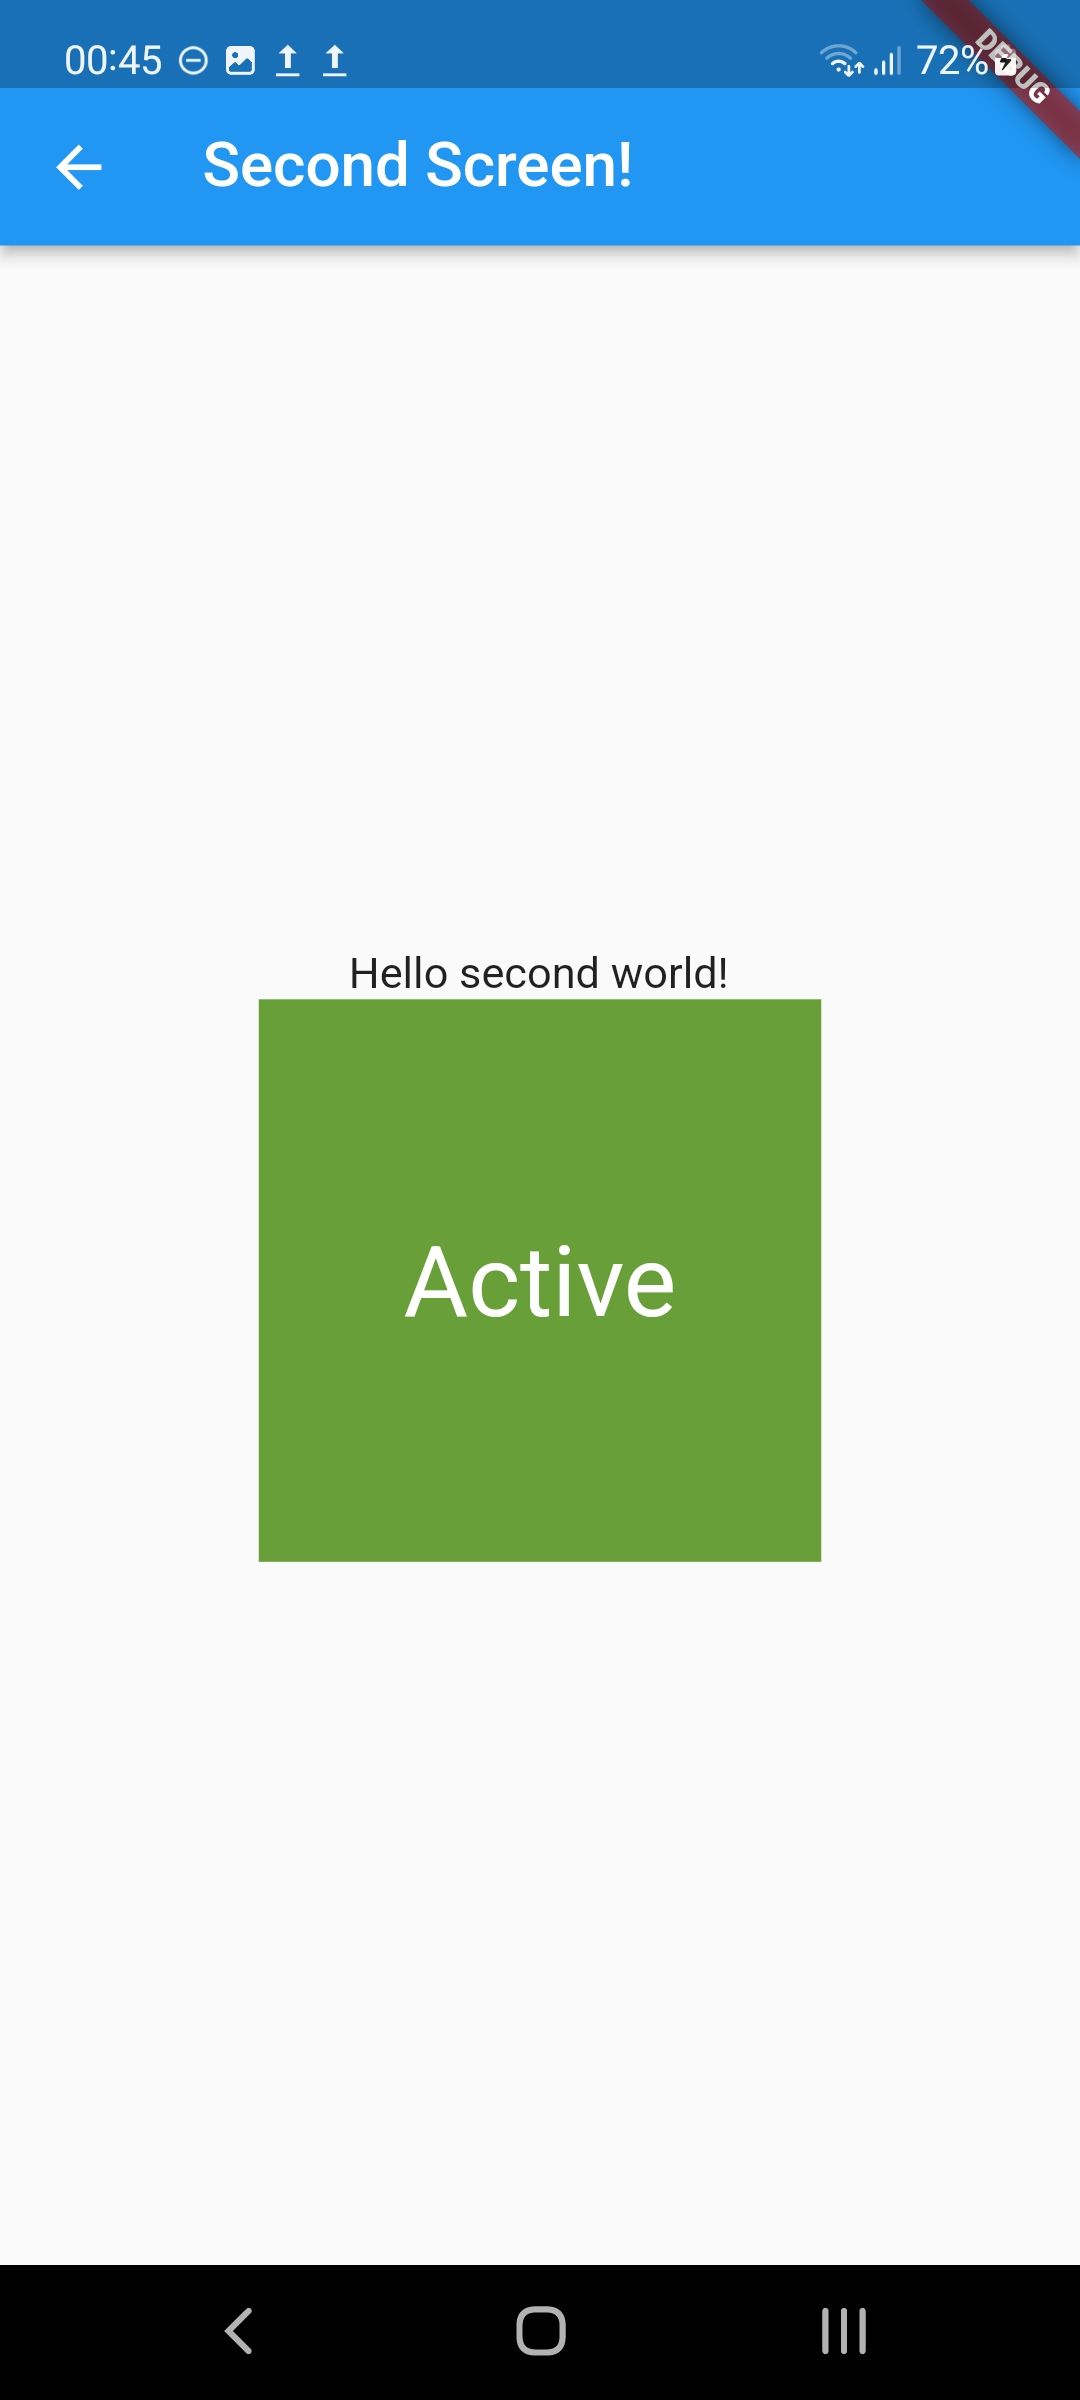
\includegraphics[width=0.5\textwidth]{images/task3-2.jpg}}
                }
            \end{figure}
        \end{column}
    \end{columns}
\end{frame}